\section{Agents as Signals}
Due to the underlying nature and motivation of FRP and Yampa, agents can be seen as signals which are generated and consumed by a signal-function which is the behaviour of an agent.  If an agent does not change, the output-signal should be constant and if the agent changes e.g. by sending a message, changing its state,... the output-signal should change as well. A dead agent then should have no signal at all.
The question is if the agents of our agent-based SIR implementation are true signals: do the dynamics stay constant when we sample the system with $\Delta t = 0$? We hypothesize that our agents are true signals, thus they should not change when time does not change because they are completely time-dependent and rely completely on time-semantics. When actually running the simulation with $\Delta t = 0$ one gets the results as seen in Figure \ref{fig:sir_abs_zero_dt}.

\begin{figure*}
\begin{center}
	\begin{tabular}{c c}
		\begin{subfigure}[b]{0.5\textwidth}
			\centering
			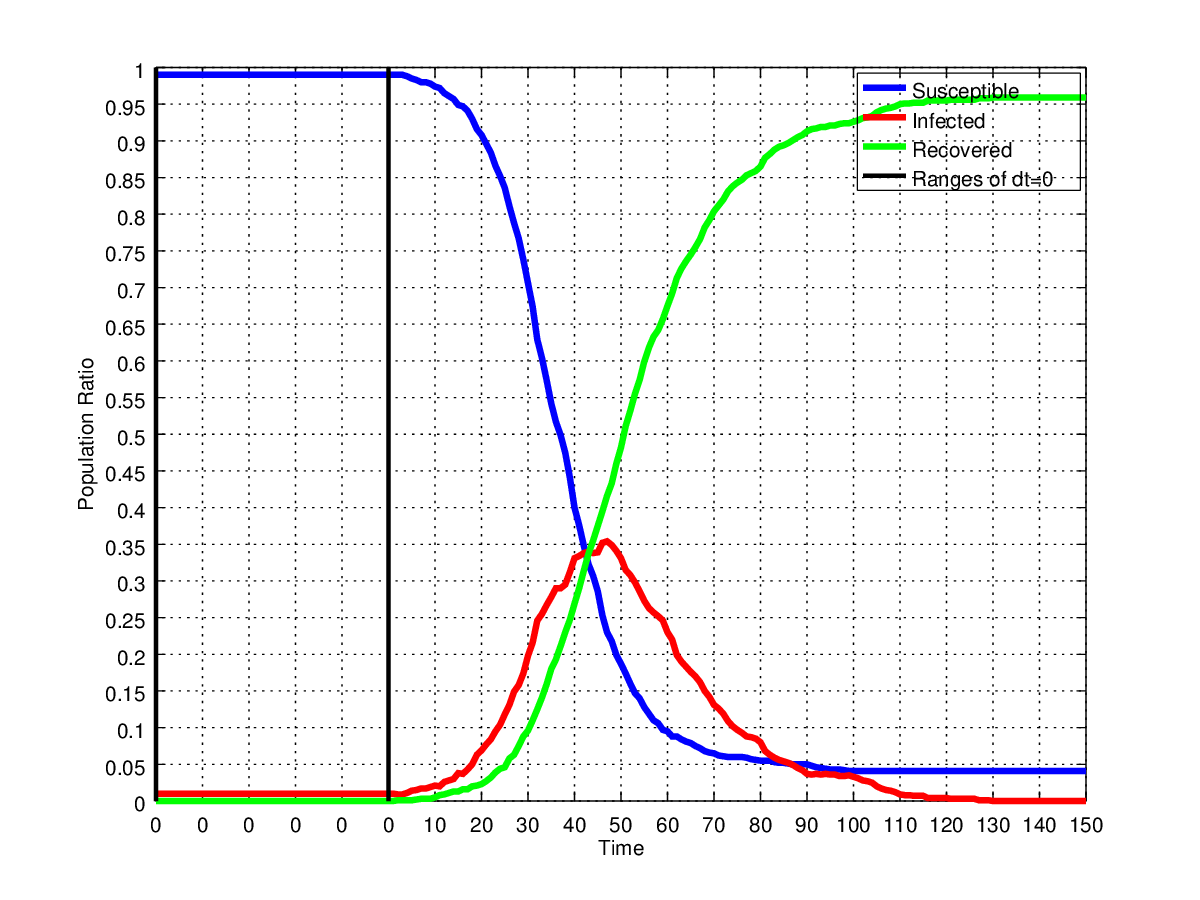
\includegraphics[width=.8\textwidth, angle=0]{./shared/fig/dtzero/SIR_ABS_zeroDt_start.png}
			\caption{$\Delta t = 0$ from step 0 to 50.}
			\label{fig:sd_plot_10dt}
		\end{subfigure}
	
		& 
		
		\begin{subfigure}[b]{0.5\textwidth}
			\centering
			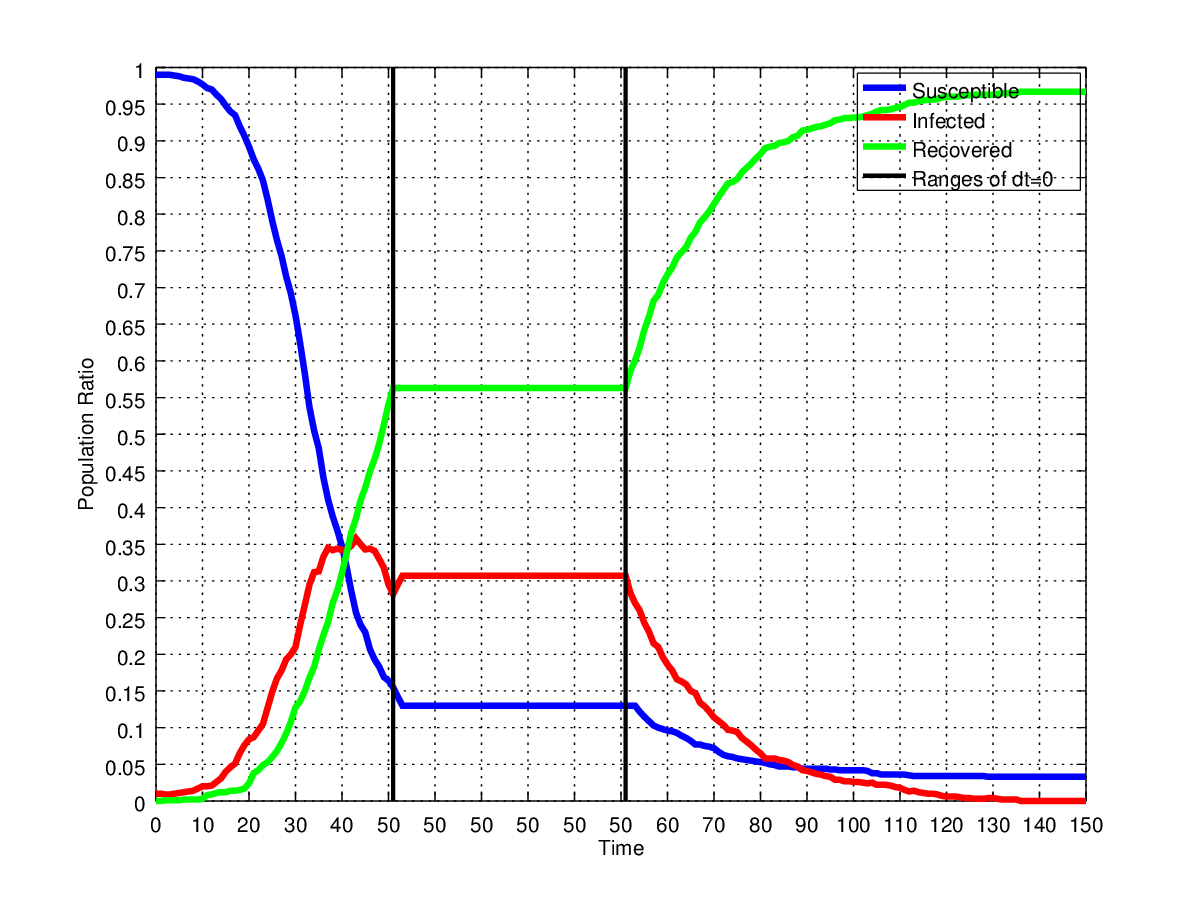
\includegraphics[width=.8\textwidth, angle=0]{./shared/fig/dtzero/SIR_ABS_zeroDt_mid.png}
			\caption{$\Delta t = 0$ from step 51 to 101.}
			\label{fig:sd_plot_0.01dt}
		\end{subfigure}
	\end{tabular}
	
	\caption{Dynamics of agent-based SIR implementation of 1,000 agents running with $\Delta t = 1$ with ranges of $\Delta t = 0$ marked with two vertical black lines.}
	\label{fig:sir_abs_zero_dt}
\end{center}
\end{figure*}

As can be seen  the dynamics are becoming constant \textit{but} with a minor delay: infected increases a bit while susceptible decreases as can be seen in Figure \ref{fig:sir_abs_zero_dt_zoom}. This is due to the delay of message delivery which takes one $\Delta t$, independent of its value - messages are also delivered when $\Delta t = 0$. Only message-generating functions, which depend on non-zero $\Delta t$ to generate messages, will then stop generating messages. Reactive functions which act on incoming messages can still create change as they do not rely on time-semantics but just on the discrete event of a message arrival - which is the case in the transition from susceptible to infected.

\begin{figure}
	\centering
	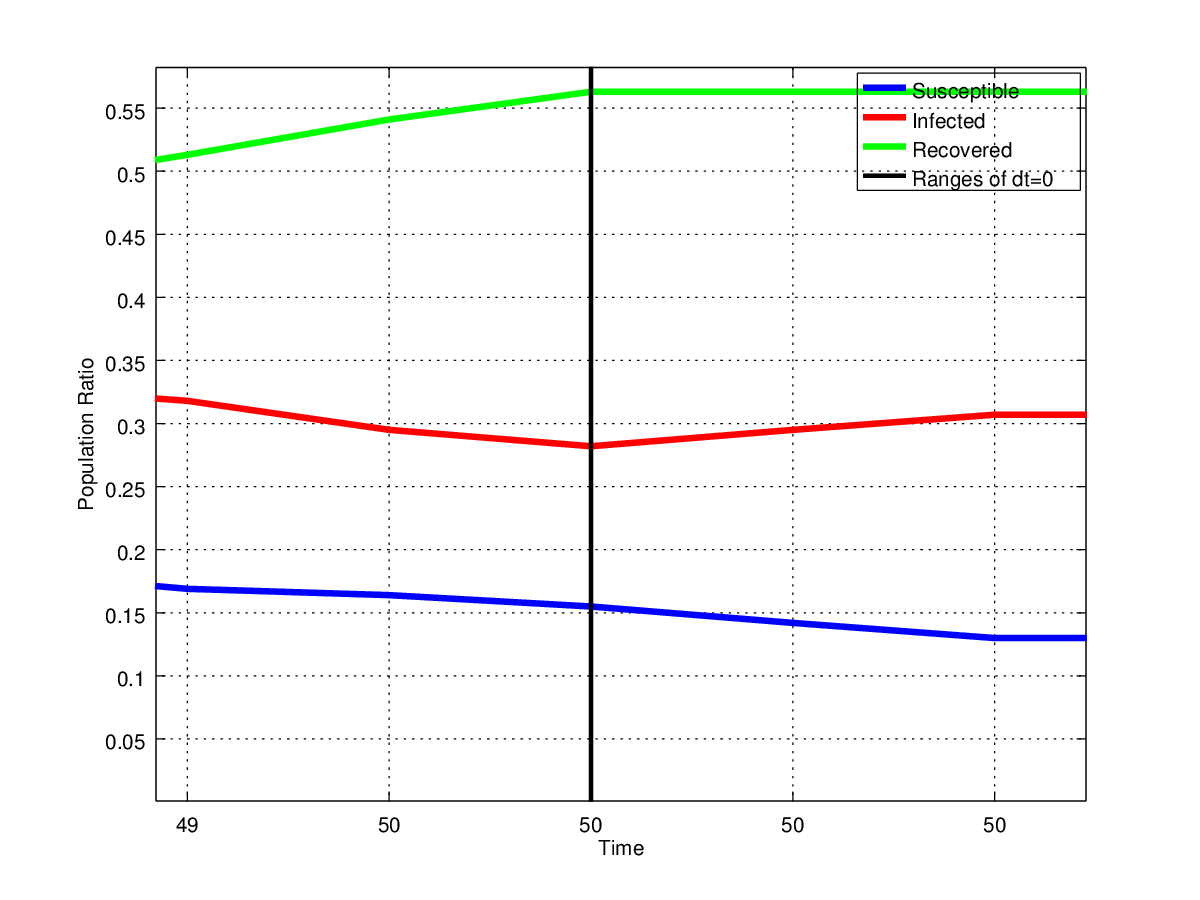
\includegraphics[width=.4\textwidth, angle=0]{./shared/fig/dtzero/SIR_ABS_zeroDt_mid_zoom.png}
	\caption{Zoom-in to step 51, marked with the black line from where on $\Delta t = 0$ for the next 50 steps. The recovered ratio stays constant but a few agents get infected even \textit{after} having switched to $\Delta t = 0$ which happens due to the message delivery lag. After all messages have been delivered, the signal stays constant until non-zero $\Delta t$ are turned on again.}
	\label{fig:sir_abs_zero_dt_zoom}
\end{figure}

Note that agents of models with no time-semantics won't exhibit this behaviour - the dynamics will change even in case of $\Delta t = 0$ as agents act on every update and don't care about $\Delta t$ and just assume that every update occurs after $\Delta t$ independent of the actual value of it. We implemented the function \textit{doRepeatedlyEvery} which allows to transform a time-agnostic agent-behaviour into one. It is built on Yampas \textit{repeatedly} function and has the following signature:

\begin{minted}[fontsize=\footnotesize]{haskell}
doRepeatedlyEvery :: Time -> AgentBehaviour -> AgentBehaviour
\end{minted}

This function takes a time interval and an agent behaviour signal-function and returns a new agent behaviour signal-function which runs the argument signal-function every time-interval. Note that this function is subject to sampling issues. When the time-interval is very small one needs to run the simulation with a $\Delta t \leq Time$ otherwise the dynamics would show delayed activation of the agent behaviour.